\documentclass{standalone}
\usepackage{tikz}
\usetikzlibrary{positioning, shapes.geometric}

\definecolor{mygreen}{RGB}{0,176,80}
\definecolor{myblue}{RGB}{0,112,192}
\definecolor{myyellow}{RGB}{255,220,0}
\definecolor{myred}{RGB}{237,28,36}
\definecolor{mylightblue}{RGB}{173,216,230}

\begin{document}
	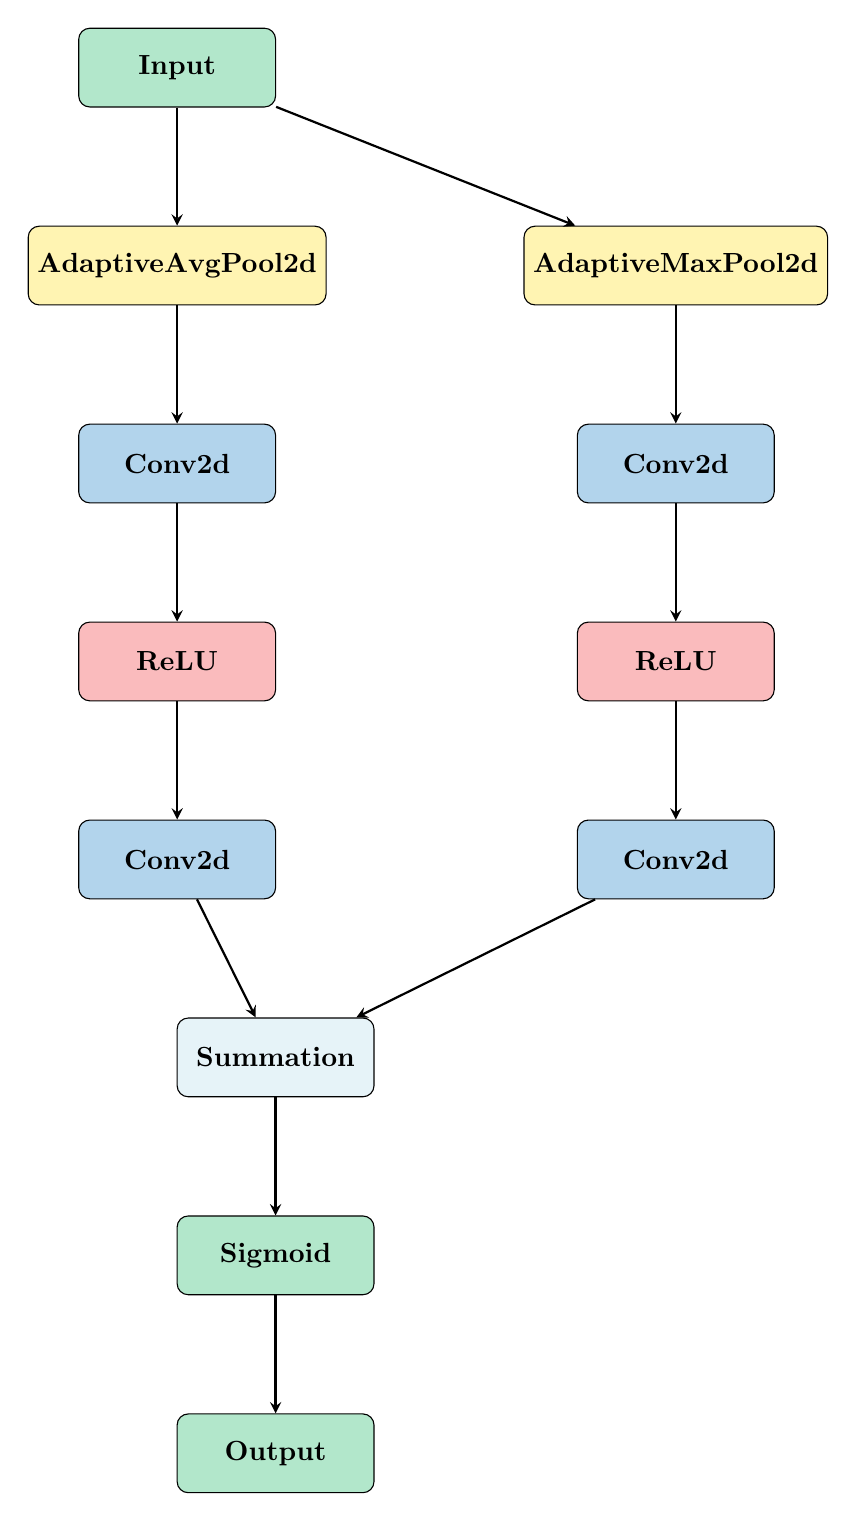
\begin{tikzpicture}[
		node distance=1.5cm and 2.5cm,
		box/.style={rectangle, draw, minimum width=2.5cm, minimum height=1cm, text centered, rounded corners, font=\bfseries},
		arrow/.style={thick,->,>=stealth}
		]
		
		% Nodes
		\node[box, fill=mygreen!30] (input) {Input};
		\node[box, below=of input, fill=myyellow!30] (avgpool) {AdaptiveAvgPool2d};
		\node[box, below=of avgpool, fill=myblue!30] (fc1) {Conv2d};
		\node[box, below=of fc1, fill=myred!30] (relu1) {ReLU};
		\node[box, below=of relu1, fill=myblue!30] (fc3) {Conv2d};
		
		\node[box, right=of avgpool, fill=myyellow!30] (maxpool) {AdaptiveMaxPool2d};
		\node[box, below=of maxpool, fill=myblue!30] (fc2) {Conv2d};
		\node[box, below=of fc2, fill=myred!30] (relu2) {ReLU};
		\node[box, below=of relu2, fill=myblue!30] (fc4) {Conv2d};
		
		\node[box, below=of fc3, xshift=1.25cm, fill=mylightblue!30] (add) {Summation};
		\node[box, below=of add, fill=mygreen!30] (sigmoid) {Sigmoid};
		\node[box, below=of sigmoid, fill=mygreen!30] (output) {Output};
		
		% Arrows
		\draw[arrow] (input) -- (avgpool);
		\draw[arrow] (input) -- (maxpool);
		\draw[arrow] (avgpool) -- (fc1);
		\draw[arrow] (maxpool) -- (fc2);
		\draw[arrow] (fc1) -- (relu1);
		\draw[arrow] (fc2) -- (relu2);
		\draw[arrow] (relu1) -- (fc3);
		\draw[arrow] (relu2) -- (fc4);
		\draw[arrow] (fc3) -- (add);
		\draw[arrow] (fc4) -- (add);
		\draw[arrow] (add) -- (sigmoid);
		\draw[arrow] (sigmoid) -- (output);
		
	\end{tikzpicture}
\end{document}
